\chapter{Literature Survey and Methodology}
Established recommendation systems face numerous security threats, plus privacy invasions and data breaches. Their distributed architecture involves multiple parties and data sources, increasing the risk of privacy violations. These security issues are extremely serious; any privacy violation may undermine user trust and dent the platform's or enterprise's reputation. Users who feel that their privacy has been violated are likely to be hesitant to give personal information or even interact with the recommendation system. This means the information will not be available and user satisfaction will be low. Besides, breaches of privacy can put the platform or business in danger of legal and regulatory action, such as fines and lawsuits \cite{ref19}.

\section{Brief Overview of Recent Literature}
\subsection*{Overview of FL-based Recommendation Systems}
To address privacy risks, Google launched federated learning in 2016 \cite{ref20}. Using this paradigm, the recommendation model can tap into a very large corpus of data from different sources, regardless of location or device type. The distributed architecture allows the model to use a more heterogeneous dataset during training by avoiding dependency on a single server. The ability of federated recommendation systems to combine the ideas of many users enables them to better understand users' interests, habits, and activity patterns, which can subsequently enable them to make more diverse and accurate recommendations. The research focuses on recommendation systems in a Federated Learning environment. The literature review comprises of topics such as cross-domain recommendation (CDR) systems, advanced methodologies, security challenges, traditional federated learning--based recommendation techniques, and federated cross-domain recommendation systems, as revealed in Fig. 2.1. To demonstrate the proposed approach, an emotional intelligence--based case study on book recommendations is presented, in which Movies, Song(Music), Books, and Games are the goal domain, and emotions are the source domain. Additionally, the review explores emotion prediction within a Federated Learning setting. The recommendation techniques are overviewed in this section.

\subsection{Conventional Approach to FL Recommendation System}
In a time of information overload, recommender systems are useful in helping users with relevant and well-targeted suggestions. This is vital in improving search results and the overall quality of the recommendation. At the same time, the privacy and security of user data should be ensured.

\begin{figure}[H]
  \centering
  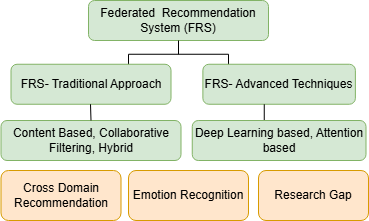
\includegraphics[width=0.8\textwidth]{figures/image12}
  \caption{Figure 2.1 Literature Review Organization}
  \label{fig:ch2_f1}
\end{figure}

Therefore, Ben Tan et al. developed FedRecSys, which supports various online applications, such as item recommendations, content, and online ads \cite{ref20}. The procedure and its employment are available under a free license. This work presents a Federated Recommender System (FedRecSys) designed to tackle security and privacy issues in online recommendation platforms. FedRecSys leverages a federated learning system in which several parties collaborate to train models while keeping user data decentralized on local devices. When deployed in real-world scenarios and integrated with many leading recommendation algorithms, the system shows improved click-through rates (+11\%) and longer average reading times (+22\%). Real implementations have proven successful in content recommendation applications.

To enhance the recommendation system’s accuracy, Su and Guanyi proposed a federated online learning model to encourage knowledge sharing. For mobile social networks, they unveiled a recommendation algorithm. To encourage customers to take part in model training, which would increase both their and the third party's (TTP) utilities, they devised a contract-based incentive structure \cite{ref21} .

FedSPLIT, an implementation of federated collaborative filtering (CF) that does not require supervision and employs NMF joint factorization \cite{ref22}. To generate one-of-a-kind recommenders, first, clients execute local CF concurrently. The next step is to tell the processor to use joint factorization to retrieve global item patterns while protecting each client's local items' privacy by analyzing them for patterns and biases. This is followed by pattern aggregation via knowledge distillation, and then the results are shifted to each participant to modify their local models.

The writers discussed concerns about the impact of recommendation algorithms on users' privacy. It is possible to make suggestions without divulging private information. They introduced an algorithm for federated recommendations, FedeRank (https://split.to/federank). Different devices use different factorization models. To train this model, the central server and federated clients operate in tandem. Users have discretion over the amount of information they share and FedeRank conducts recommendation computations in a distributed manner. Extensive experiments demonstrate that, in comparison to SOTA algorithms, FedeRank achieves higher accuracy with very little user data sharing \cite{ref23}.

Ensuring fairness, or uniformity, in the performance of recommendations among federated learning participants is the main topic of the article by G. Lin et al. Their suggested framework, Cali3F, connects the neighborhood to a federated CF recommendation system in order to do this. Training both local and global models is achieved through a multitask learning framework. FedRec is a federated learning-based recommendation system designed to protect privacy while predicting customer ratings. Although traditional collaborative filtering methods risk exposing user preferences, FedRec addresses this by keeping rating activities private. The framework introduces two main approaches: hybrid filling (HF), which replaces unrated items with projected ratings based on negative feedback; and user averaging (UA), which provides an average rating for unrated items. FedRec reduces privacy risks and computational costs while maintaining accuracy comparable to non-federated models, based on tests using the MovieLens 100K and 1M datasets. The work highlights FedRec's versatility and its relevance to models such as SVD++, beyond Probabilistic Matrix Factorization (PMF). As a result, both computational speed and fairness are improved \cite{ref24}.

The study by Liang F et al. looked at privacy-aware suggestions with direct comments. The authors present FedRec++, an innovative lossless FRS that leverages filtering clients to remove noise generated by virtual ratings assigned to a random sample of items. Furthermore, the authors examined FedRec++'s privacy features and revealed that it provides robust privacy to users\cite{ref25} .

The researchers provide detailed explanations of numerous methods and advancements in this area. In their chapter, Yang, L. Tan, B., and others describe federated recommendation systems in great detail. The horizontal, vertical, and transfer learning are the pillars of federated learning---form the basis of this summary. User-item sharing scenarios determine the classification (feature space). The difficulties of developing federated recommender systems are discussed. Additionally, federated recommendation systems are categorized at both the algorithm and system levels \cite{ref12}.

Both stakeholders and recommender systems benefited from the use of FL by Saikishore Kalloori et al. To form a federated recommendation model cooperatively using training data from the client's or other stakeholders' systems, they devised a federated learning approach that averages model updates. Two widely used algorithms, including Neural Collaborative Filtering and Bayesian Personalized Ranking, were used to implement this strategy \cite{ref26}.

The initial federated Collaborative Filter implementation was presented by Muhammad Ammad-ud Din et al., and it updates models using a stochastic gradient method. A classic machine learning case study is presented in the paper, which analyzes a customized recommender system that relies on implicit user input. Due to its simulation nature, the system requires further investigation into the actual case of clients' asynchronous data transfer \cite{ref9}.

The authors examined the key challenges and recent advancements in federated recommendation systems in \cite{ref28}.

\subsection{Enhanced Techniques for FL Recommendation Models}
In an attempt to use user-item interaction to generate new insights using additional information of the user , Wang Q. et al. \cite{ref13} designed PrivRec, a deep neural network-based recommendation engine to deal with the issue of the asynchronous nature of data transmission. They proposed a successful, practical meta-learning approach for PrivRec that enables FL to support data heterogeneity and idle users in recommender systems. In addition, they enhanced the privacy of PrivRec by introducing user-level differential privacy features, which reduced the likelihood of revealing sensitive information to malicious FL clients. In turn, DP-PrivRec became a more resilient and secure model.

To protect sensitive information without affecting the training process or the model's performance, Liu Yang et al. proposed a tailored masking strategy to mitigate the computational overhead of DP-based systems. By applying it to the FedMMF algorithm, they have proven that this method is effective in the recommendation scenario. In addition, FedMMF demonstrates better performance, both in theory and in practice, by using an adaptive secure aggregation algorithm. \cite{ref30}

Continuing in the same way, Amir J. et al. have presented an FL strategy for recommender systems that is both simple and effective in improving customization. Related meta-learning algorithms are also discussed. The outlined method outperforms the existing FL recommenders in real-world scenarios while being simpler to implement. The authors tested the algorithms' ability to forecast user ratings using benchmark data and evaluated their performance experimentally using RMSE. Encryption is necessary to guarantee the user's anonymity when reconstructing their gradients or parameter modifications. \cite{ref31}

For session-based RNN modeling, Yang, L. et al. have proposed multiple parallel RNN architectures that incorporate click data and attributes, such as linked images and text. They went a step further by suggesting improved training methods for P-RNNs beyond the current standard. The results demonstrate that compared to featureless session models, p-RNN architectures perform significantly better when trained correctly. By comparison, session-based models yield better results than the item-wise average.\cite{ref32}

This research introduces a Privacy-Preserved Recommender System Framework (PPRSF) designed to manage the privacy-personalization trade-off in traditional recommender systems based on Federated Learning (FL). By separating public and private user data, PPRSF reduces privacy risks while maintaining recommendation quality, enabling model training without centralized data collection. The framework features a four-layer hierarchical structure: the Recall Layer (server-side) pre-filters candidate items; the Ranking Layer (client-side) refines recommendations with private data; the Re-Rank Layer (server-side) enhances diversity and fairness; and the Service Layer (client-side) presents results and collects new interactions. FedAvg facilitates the pooling of locally trained ranking algorithms across the globe.

A privacy-protecting FL method for top-N POI (points of interest) ideas, FedPOIRec, that uses users' social network data was introduced by Perifanis, Vasileios, Drosatos, et al. to raise awareness of the technology. The FedPOIRec architecture states that clients retain local data and updates while the server aggregates them. By letting users share learned parameters, FveriedPOIRec also facilitates knowledge exchange among friends. \cite{ref32}

Combining social impact with data privacy, FedPOIRec is an FL system developed to preserve privacy in POI recommendations. Secure Multiparty Computation (SMC) and Fully Homomorphic Encryption (FHE) are used for secure model aggregation and social feature integration, unlike traditional centralized models that store user data on local devices. FHE has significant processing costs, and the system encounters issues with sparse data and cold-start users. Other unresolved challenges include adversarial robustness and scalability on devices with limited resources \cite{ref32} \cite{ref34}.

\subsection{Safeguarding Federated Recommendation Systems}
The researchers integrate user preferences for federated computation with a program that protects privacy and leverages all features of the CKKS homomorphic encryption system \cite{ref34}. With the FGBDT system, MNOs and HPs can engage in collaborative modeling while protecting users' privacy without compromising data exchange. Better user classification using combined MNO and HP data is a potential outcome of using the suggested system in healthcare recommendation apps \cite{ref35}.

I. Guillén et al. discussed a privacy-preserving recommender system (RS) using Federated Learning (FL) to address growing ethical and legal concerns about collecting user data. Unlike other centralized RS models, the proposed method stores raw user data locally, preserving both recommendation accuracy and privacy. Instead of directly merging synthetic user profiles, the system generates them through a consensus-based aggregation process, thereby avoiding privacy issues by retraining models rather than merging them directly. The system was tested with GreenSoul and Prolific datasets (N=678) and evaluated using the Normalized Distance-Based Performance Measure (NDPM), employing four Raspberry Pi devices and an NVIDIA Jetson Nano as the aggregation server. Results indicate that, even with reduced communication and processing costs, the FL-based RS delivers accuracy comparable to or better than centralized approaches. Additional privacy protections are provided by a hybrid encryption system that secures model updates \cite{ref2}.

Based on matrix factorization, J. Zhang and Y. Jiang \cite{ref35} presented a hybrid, clustered, vertical, federated matrix recommendation method. They modify the prediction score of the federated matrix factorization recommendation model by adding a user-clustering strategy. This approach makes it easier to cluster users' latent factor vectors. This approach guarantees that user rating information remains within each recommendation system while enabling the proper study of user-item correlations. Using homomorphic encryption, consumers' private data is protected. M. Dogra et al. introduce a novel approach to Recommender Systems (RS) built on Federated Learning (FL). The items and users in this method are encoded in a fixed-size format that remains constant regardless of their quantity. This method works well for large-scale RS applications and uses little memory. Using a Next App Recommendation use case, the framework has been proven to deliver performance on par with previous solutions while consuming much less memory\cite{ref36}.

\subsection{Cross Domain Recommender Systems}
CDR methods can be categorized by their focus on content, features, embedded transformation, ratings, or a mix of these. To integrate attention mechanisms at the item and domain levels, the authors proposed a neural network method called NATR.  To protect privacy, the Neural Attentive Transfer Recommendation (NATR) model employs attention mechanisms at the item and domain levels to extract proper collaborative filtering (CF) signals from transported embeddings. Evaluated with MovieLens-Netflix and iQiyi-Tencent Video datasets, NATR outperforms traditional cross-domain models (CMF, ItemCST), achieving up to 18.94\% higher HR@10 and resolving cold-start problems for items. However, the research has limitations, including embedding dimensionality inconsistencies, scalability issues in large-scale environments, cold-start user problems, and security vulnerabilities to adversarial attacks. Transferring item embeddings from the secondary domain helps address issues in CDR learning by preventing user privacy leakage. No research has been conducted on the approach's scalability  \cite{ref37}.

To create user and object latent factors, the researchers in  \cite{ref38} presented a matrix factorization-based approach that subsequently employs deep neural networks to map these factors across domains. This paper proposes a deep learning module for CDR, CSR, and CDCSR. It maps user and item latent variables across domains using a DNN and MF, then generates them. It includes benchmarking aspects that account for rating sparsity to ensure a more accurate mapping.   When measuring MAE and RMSE, the model outperforms SOTA techniques on the Douban, Netflix, and MovieLens datasets.   The approach ignores real-time deployment, assumes a fixed mapping function that would not be appropriate across somewhat distinct domains, and omits emotion-based features.   Training the DNN also incurs computational expenses that affect scalability; the model does not fix the cold-start problem for new users or objects.

Other CDRs are working on dual targets. \cite{ref39}, \cite{ref40}  \& \cite{ref41}  . Unlike conventional single-target CDR systems, the DTCDR framework.\cite{ref39} It is a new Dual-Target Cross-Domain Recommendation (CDR) system that improves recommendation accuracy across both domains. It uses Multi-Task Learning (MTL) to distribute user embeddings among domains, hence improving suggestions in both richer and sparser environments. Three embedding combination techniques---concatenation, average pooling, and max-pooling---are investigated to improve information transmission.

The system produces document embeddings (Doc2Vec) and rating embeddings (NeuMF and DMF), and combines data from several sources, including user profiles, ratings, reviews, item data, and tags. With up to 13.73\% improvement in HR@10 and 18.83\% in NDCG@10, experiments on MovieLens and Douban datasets reveal that DTCDR performs better than single and cross-domain models. Still, specific difficulties exist. The computational complexity of MTL-based embedding sharing raises scalability concerns and makes large-scale installations difficult. Cold-start users---who could benefit from meta-learning---are not explicitly addressed by the approach. Furthermore, no adaptive process is proposed to select the optimal embedding combination.

\subsection{Federated Approach to Cross-Domain Recommendations}
The research goals in \cite{ref42}, \cite{ref43}, \cite{ref44}, \cite{ref45},\cite{ref46}, \cite{ref47}, \cite{ref48} , and \cite{ref8} are to address data privacy and the problem of cold-start users in recommendations. They accomplish this by enhancing recommendations using a domain with rich information. The confidentiality of user information is preserved throughout the process of resolving these issues. To guarantee privacy in CDR, the authors presented a Federated framework. The suggested techniques acquire user and item embeddings by training a standard recommender model on all client devic42es. After that, each client sends its weights to the central server. Local differential privacy is a privacy protection scheme that can protect user information by perturbing the weights before uploading gradients. The similarity between a user's embeddings in the two domains is further narrowed by performing embedding transformations at the server. The methods are a privacy-saving and consistent CDR technique with valuable results in privacy assurance and personalized suggestions. FedCDR, which is specifically built around federated learning, places more importance on privacy, but it deals with the problem of sparse data and cold-start users or items in cross-domain recommendation models. FedCDR also allows recommendation-model training to be performed on the user's device, compared to traditional CDR models that use a centralized data warehouse, which helps avoid exposing raw data to unauthorized access. It addresses privacy breaches by adding noise to gradients before sending them to the central server and uses Local Differential Privacy (LDP). In addition, the federated aggregation system, FedAvg, guarantees that raw data are never sent but only encrypted model updates are. Experiments on Douban datasets demonstrate that FedCDR is more efficient than current privacy-saving methods, such as CCMF, and is equally efficient in terms of recommendation quality as centralized models. FedCDR with an appropriate distribution of privacy budget ($\epsilon$), gradient clipping ($\delta$) and noise magnitude ($\lambda$) displays stability under different percentages of cold-start users, thus attaining the ideal privacy-accuracy trade-off \cite{ref42}

The paper presents a Federated Cross-Domain Social Recommendation (FCSR) algorithm, which enables the privacy-sensitive cooperation between social service platforms (SSPs) that store the information in social networks and information-oriented websites (IOWs) that store the information on feedback on users. Conventional cross-domain advice relies on data gathered centrally, thus increasing privacy-related issues, and in most cases, this can be very impractical because of limitations to accessing the data. The authors leverage Federated Learning and use two major privacy mechanisms: the Random Response Mechanism (RRM), which attenuates the perturbation of social contacts, and the Matrix Confusion Method, which encrypts user feature vectors to enable updating features without revealing individual information. The system enhances computational efficiency by decomposing sparse matrices using lower-upper (LU) decomposition, which eliminates the complexity in solving large-scale linear systems. Experiments with FilmTrust, CiaoDVD and Epinions show that FCSR is significantly more accurate than incumbent federated recommendation systems (FedMF, FedGNN, FeSoG) and keeps users private  \cite{ref44}.

CDR is one way to address the cold-start user or item issue in conventional recommender systems. This approach uses exchanges between the source and target domains that allow cold-start users to see personalized suggestions. As much as the present CDR techniques are popular, they rely on a shared-preference bridge, where they share data with each user, thus not capturing the unique and diverse preferences of each user \cite{ref50}.  Moreover, they need direct two-way data exchange between servers and clients, which increases privacy concerns. To overcome such difficulties, the authors proposed a user-specific cross-domain preference bridge based on federated meta-learning. They used FL to train a preference bridge that sums local stored data and model parameters. This plan does not compromise the privacy of users and improves the effectiveness of CDR \cite{ref45}.

IoT innovations boost the rapid increase in large volumes of data. From such large datasets, a cross-domain recommendation engine is effective in determining objects that a user likes. Nevertheless, three issues can be encountered when implementing a cross-domain recommendation system across dispersed IoT devices. Embeddings of currently popular items tend to have a popularity bias. Also, most existing techniques rely on shared-interest channels to convey user preferences. People have different tastes, and thus it is reasonable to expect different users and interests. The information received from dispersed IoT devices can also pose a privacy risk. This paper presents FedBP, a federated FedCDR that integrates a bias eliminator and a custom extractor system to improve recommendation accuracy in cold-start situations. All embedding directions are elongated during training with the help of a bias eliminator, and each route registers only specific information and is neutral in terms of popularity. In addition, a tailored extractor will match users' individual preferences in the domains. This system is trained in a federated architecture and secures data privacy using local differential privacy.\cite{ref46}

The paper in \cite{ref47} introduces a new multi-view federated learning framework, Fed-FR-MVD, developed for data-diverse, privacy-conscious e-commerce environments to increase recommendation accuracy. Current federated learning (FL) methods have issues related to data heterogeneity, inefficient feature extraction, and noise sensitivity, whereas concerns related to data privacy have long plagued traditional centralized recommendation systems. To address these issues, Fed-FR-MVD integrates an item- and user-view-based multi-view architecture that uses a Feature Rescaling (FR) method. FR module is a dynamic feature weighting method that focuses on relevant characteristics and suppresses noise. On the multi-view complex data, a deep structured semantic model (DSSM) can be used to learn a better representation. Experimental findings on Amazon data indicate that Fed-FR-MVD is more robust to noise rates of 5\%-15 \%, and is stronger in comparison to techniques based on single or multiple views by 12\%-18 \% \cite{ref47}.

In \cite{ref48}, an original method of Privacy-preserving Cross-domain Recommendation (PCDR) has been introduced to address privacy leaks in domains and data heterogeneity in federated cross-domain recommendation (FCDR). PFCR uses universal item representations based on text content descriptions, unlike previously presented studies that use user identity overlap to align domains, which puts users at risk of privacy issues. A vector-quantized item representation method uses text to produce discrete codes, which allows efficient semantic matching across domains. Privacy preserving aggregation employs federated averaging (FedAvg) where the gradients of items are shared but user-specific ones remain local \cite{ref48}.

CDR has been used extensively to reduce data sparsity because it cross-domain transfers information. Current studies combine federated learning and CDR due to the potential for compromised data privacy when direct information is exchanged.

However, these methods require homogeneous models across domains and incur significant communication costs, which limit the adoption of federated learning. This paper presents a “one-shot” federated cross-domain ensemble learning system called FedOCD. There are two primary parts to FedOCD: the first is source-domain modeling, which uses source-domain data to learn user embeddings while protecting their privacy via Local Differential Privacy (LDP); the second is the target-domain ensemble, which uses source-domain user features to enhance recommendation performance. FedOCD significantly improves performance, according to experimental results on benchmark datasets. \cite{ref49}

To handle cold-start and data sparsity challenges, CDRs are becoming increasingly crucial for delivering personalized data across disciplines such as e-commerce and healthcare. Accurate recommendations in one area are made possible by using user profiles and adequate ratings in another. Many highly rated places are hesitant to let third-party recommendation systems or domains access user ratings because of privacy concerns. Hence, a privacy framework is required for cross-domain data transfers. To address privacy and cold-start issues in CDR systems, this study presents the CrossRec-Hybrid Federated Transfer Learning (CrossRec-HFTL) platform. It leverages user-item interaction in an annotated source domain to make recommendations in a non-annotated target domain, combining adversarial domain adaptation with federated learning. Simulation findings show that CrossRec-HFTL achieves higher suggestion accuracy than the baseline and modern recommendation systems, with a comparatively low RMSE of 0.82 and MAE of 0.58. This demonstrates the model's improved privacy protection and its great performance in cold-start scenarios \cite{ref8}.

\subsection{Emotion Recognition and Federated Learning}
Researchers in both education and business are always interested in emotion recognition and sentiment analysis. Since federated learning is a relatively new tool, much work remains to be done on emotion recognition. Obtaining multimodal data for emotion detection without sensors and IoT devices is difficult; therefore, text-based emotion recognition has attracted significant attention from researchers in both academia and industry.Audio (e.g., voice emotion detection), visual (e.g., facial expression recognition), and textual data, collectively called multimodal data, have been the main focus of researchers in the works cited as \cite{ref51} and \cite{ref52}. In a federated setting, Nandi et al. \cite{ref52} established a model, Fed-ReMECS, that classifies real-time emotions from physiological measurements obtained from data streams generated by wearable sensors. V. Tsouvalas et al. used a semi-supervised federated learning approach to create speech-emotion recognition in \cite{ref53}. They proved that the addressed method improved emotion identification by 10.0\%. By combining a FedL strategy with a privacy-preserving CNN-based audiovisual model for emotion recognition, Simic et al. achieved a 2\% improvement in accuracy \cite{ref54}.

\begin{figure}[H]
  \centering
  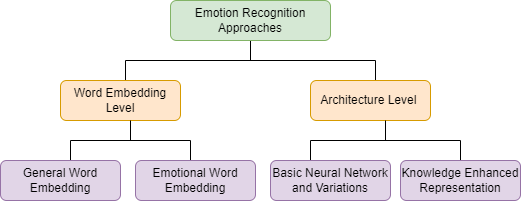
\includegraphics[width=0.8\textwidth]{figures/image13}
  \caption{Figure 2.2 Emotion Recognition Techniques}
  \label{fig:ch2_f2}
\end{figure}

Emotion recognition in text can be achieved in numerous ways. This encompasses several levels of deep learning methods, including training, architectures, and word embeddings, as shown in Figure 2.2  \cite{ref55}.

A mathematical process called ''word embeddings'' can uncover hidden connections between words. Word embeddings are versatile and can be used for both general and emotional purposes. Distributed semantic modeling is the foundation upon which they rest. We have two broad word-embedding models: Word2Vec. \cite{ref56} and Glove \cite{ref57}. According to ELMO \cite{ref58}, Advanced pre-trained models include GPT, BERT, and others alike. Emo2Vec \cite{ref59}, Emoji2Vec \cite{ref60} , and DeepMoji  are examples of models that have already been trained (pre-trained) to process emotional words \cite{ref61}.

Researchers have suggested several neural network models for extracting semantic and sequence information. The use of long short-term memory (LSTM), pre-trained recurrent neural networks (RNNs), gated recurrent units (GRUs), and similar networks is effective. \cite{ref62}.

Many people also use an attention-based approach to speed up training and improve performance. GRU-based attention is used in hierarchical attention. \cite{ref63}, and LSTM is used in TreeLSTM \cite{ref64}. The network collaborative models are composed of several separate models that work together to produce strong, complete models. \cite{ref55}.

For a more thorough understanding, knowledge-enhanced representations take into account prior information, such as language patterns, emotional lexicons, and other commonsense knowledge about emotions. \cite{ref65}. Affective computing includes the study of interrelated attitudes and emotions. Researchers have widely used the FedL method to improve sentiment analysis, data privacy, and isolation.

Ahmad et al. researched aspect-based sentiment analysis (ABSA) \cite{ref66} \cite{ref18}. ABSA pertains to the targeting of sentiment in sentences across various disciplines. This field has made significant advancements due to developments in DL and pre-trained language models. This field is affected by concerns regarding data privacy. The authors proposed a novel approach to address this issue, introducing prompt-enhanced FL (PFL) for aspect-based sentiment analysis (ABSA). This approach combines prompt tweaking and the privacy-preserving aspects of federated learning. The authors introduced PFL-GCN, a graph convolutional network that combines PFL with BERT.\cite{ref67} In FL settings, researchers test solutions to several natural language processing (NLP) problems.\cite{ref68} Han Qin et al. investigated how aspect-based sentiment analysis (ABSA) becomes more complicated due to pattern divergence across sentences from multiple sources. Legal and privacy concerns restrict access to labeled data for all parties, even though it is available across various locations and sources.

Nuria R. et al. investigated Federated Learning in \cite{ref69}, to resolve arguments about annotations in NLP. In sentiment analysis, annotation is vital. During dataset annotation, the suggested approach treats each annotator as a federated client. At last, the model can gather labels from clients worldwide and combine them without human intervention. Discrepancies found among subject-area annotators teach the model new things. Because of its extensive use in research, FedAvg is widely used.

Large language models (LLMs) were adopted in a federated learning (FL) setting by Himkil et. al. \cite{ref70}. FL's privacy characteristics and conformity with legal norms are increasing its appeal for a variety of applications. This research looks at FL in relation to LLMs. The researchers assessed sentiment analysis using BERT, ALBERT, and DistilBERT and discovered that performance is user-dependent. Researchers need to investigate the causes of DistilBERT's increased latency as the number of clients escalates \cite{ref71}.

S. Bansal et al. used topic preference and sentiment analysis to predict personality traits in \cite{ref72}. They used LDA and LSTM models to assess user-generated content from Weibo. Our eight-figure personality forecast. This approach brings up significant privacy concerns and ethical quandaries. The writers demonstrated how to address the highlighted problems effectively. Unfortunately, there was no proof that the FL method was used for privacy control.

Another approach to identifying consumer complaints was suggested by J. Zhao et al. in \cite{ref73}, which uses a graph attention network. As a part of natural language processing, we can categorize social media complaints. This requires a central system of collecting, distributing, and processing data. This solution fails to consider privacy and decentralized data. The authors believed that by integrating a graph-attention network into the federated learning setting, they would be able to solve this issue. The global and local models can be enhanced using adaptive optimization techniques such as the Fedcomb algorithm simultaneously. In terms of complaint recognition, our strategy outperformed baseline techniques. We need to test this model on bigger datasets.

Investigating how Federated Learning (FedL) incorporates sentiment analysis and privacy preservation has been done by Sakhare N.N. et al. \cite{ref74} and Priyam Basu et al.\cite{ref75}. Within the framework of blockchain technology, the authors of \cite{ref74} investigated the spatial FedL approach for sentiment analysis of stock news. It is critical to do in-depth research on each stock before buying. When analyzing stock market fluctuations, it is essential to account for both the short-term and long-term effects of external factors, as well as corporate details. The writers used spatial federated learning (SPL) to retrieve and analyze news stories from the Economic Times' website. Concerns about confidentiality and regional differences were therefore resolved. Federations use a variety of algorithms. In order to make decisions, every federation takes into account public opinion.

The classification of financial text is addressed by FedL in \cite{ref75}. Financial data must be kept private due of its sensitivity. To train large models, this data must be properly managed. The writers used federated learning, differential privacy, and text classification models based on contextualized transfer learning. The model outpaced the SOTA transformer; though, it performs miserably on imbalanced data.

\subsection{Investigations based on review}
The research gaps identified in the traditional approach to federated learning recommendation systems are:  No direct comparison is provided between federated learning-based recommendation models and centralized recommendation models in terms of accuracy, precision, and recall \cite{ref21}, \cite{ref22} \& \cite{ref24}. A few approaches in our discussion are group-based, meaning individual users cannot directly participate without a predefined group  \cite{ref23} \cite{ref25}. Many approaches focus on a single domain \cite{ref22} \cite{ref26} \cite{ref12} \cite{ref27}. The traditional approach does not address Cross-domain recommendation. Recommendation systems are simulation-based; hence, they lose the real-world context \cite{ref27} .

The research gaps identified in advanced techniques for recommendation in Federated Learning include computational overhead concerning the use of advanced ML algorithms \cite{ref30}\cite{ref31}, cold-start issues, scalability constraints\cite{ref32} , and security vulnerabilities to adversarial attacks\cite{ref9}.

The research gaps identified in security for federated recommendation systems are: the use of different encryption techniques results in Computational Overhead and Scalability \cite{ref29}\cite{ref33}\cite{ref36}, and Real-World Deployment Feasibility \cite{ref37}.

The research gaps identified in CDR systems are: The model discussed in \cite{ref39} does not address the cold-start problem for new users or items. While the DNN improves mapping accuracy, training a deep network requires considerable computational resources \cite{ref39}, \cite{ref40}  and \cite{ref41}. All these systems rely on sharing user data across different domains for accurate recommendations \cite{ref39} \cite{ref40}, \cite{ref41} and \cite{ref42}.

The research gaps identified by Federated Cross-domain Recommendation (FedCDR) systems include: communication costs and communication overhead \cite{ref43} \& \cite{ref44} , scalability concerns, scalability challenges, cold start issues \cite{ref45}, and the ongoing challenge of real-world validation \cite{ref46}, \cite{ref47}, \cite{ref48} , \cite{ref49}, \& \cite{ref8}.

Reviewing the literature on Emotion recognition [46-66] shows that no previous implementation has addressed the challenge of deploying neural networks on mobile devices with restricted resources and bandwidth.

\section{Methodology}
The proposed research applies an organized methodology to design, implement, and evaluate a multi-objective cross-domain recommendation system within a federated learning framework.

\subsection{Overall System Design}
The system is structured into three major layers:

\begin{itemize}
    \item Local Client Layer: This layer is responsible for data processing on the local device. The local model is trained, and emotion prediction is done. The PRADO architecture is used for feature extraction and emotion classification on edge devices.
    \item Federated Aggregation Layer: The layer includes the central server, which is responsible for collecting weight parameters and aggregating them with the FedAvg algorithm to build a global model.
    \item Recommendation Layer: This layer performs cross-domain recommendation using federated transfer learning and an advanced recommender using cosine similarity-based fingerprinting.
\end{itemize}

This layered architecture ensures privacy preservation, modularity, and scalability.

\subsection{Data Collection and Processing}
\subsubsection{Data Collection}
This research utilizes two primary datasets:

\begin{itemize}
    \item GoEmotions Dataset: Contains approximately 58,000 Reddit comments, annotated with 27 emotion labels and one neutral category, and used for emotion prediction tasks.
    \item Books Dataset: This is derived from the Kaggle Books\_rating dataset. It contains approximately 10,000 curated book titles and reviews, categorized into fiction and non-fiction genres.
    \item CMU Movie Summary Corpus: 42,306 Wikipedia movie plot summaries and a rich set of movie and character metadata for NLP and recommendation research \cite{ref95}.
    \item Genius Song Lyrics Dataset: A large-scale song lyrics database and metadata set with lyrics from Genius around music, sentiment, and emotion analysis.
    \item Steam Games Dataset: This is a metadata database for more than 83,000 Steam games, comprising their genres, their developers, their release data, their pricing, and their review scores.
\end{itemize}

These datasets enable cross-domain learning by linking user emotions from social media with target domain recommendation preferences.

\subsubsection{Data Processing and Feature Extraction}
Data preprocessing includes convolution and pooling. The Projected Attention Network (PRADO) is used for feature extraction due to its efficiency on resource-constrained devices.

PRADO replaces traditional embedding layers with projection-based representations, reducing memory requirements. The model performs:

\begin{itemize}
    \item Projection-based embedding
    \item Convolutional feature extraction
    \item Attention-based weighting
    \item Text encoding
\end{itemize}

The extracted features are then used for emotion prediction and further integrated into the federated learning pipeline.

\subsection{Local Model Training}
The local model on each client is trained using the Projected Attention Network (PRADO) architecture. It captures important features from the given text input and performs emotion classification locally on each client device.

The Fig. 2.3 demonstrates the overall working of the proposed system.

\begin{figure}[H]
    \centering
    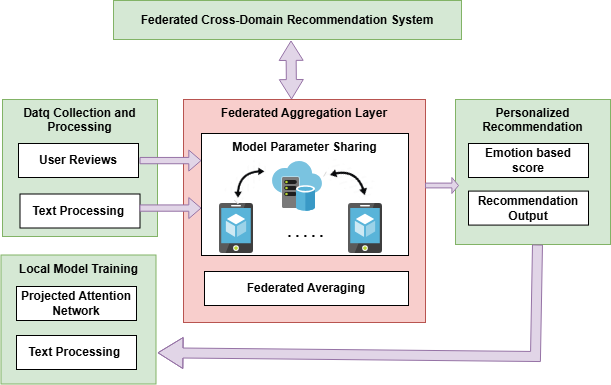
\includegraphics[width=0.8\textwidth]{figures/fig2_3_framework}
    \caption{Federated Learning Framework for Recommendation System}
    \label{fig:fed_framework}
\end{figure}

\subsection{Federated Learning \& Model Aggregation Process}
The process includes an iterative communication protocol as demonstrated in Fig. 2.3. Each client trains the model locally using PRADO. The trained model weights are sent to the central server, where they are aggregated using the FedAvg algorithm to produce an updated global model. This global model is then distributed back to the clients for the next round of training.

\subsection{Personalized Recommendation}
The aggregated global knowledge is received, which includes updated local model parameters for emotion prediction. Based on these parameters, the recommendation module generates personalized recommendations for each user across different domains using cosine similarity-based fingerprinting and random forest-based lookup.

\section{Summary}
This chapter reviews various recommendation approaches within a federated learning environment. It covers traditional methods, advanced techniques for federated recommendation systems, security concerns, CDR systems, and federated CDR systems. Each system mentioned is discussed in detail. The chapter identifies research gaps in accuracy, cold-start issues, scalability, security, and real-world deployment that motivate the proposed system.

